\chapter{Background and Related Work}
\label{chap:background}

\section{Localization Technologies}

Indoor localization encompass a wide range of technologies designed for tracking and positioning within indoor environments. This chapter provides an overview of key technologies, comparing them based on multiple factors, including whether the user needs to carry a device, accuracy, sustainability, cost, and infrastructure requirements. Various methods such as GPS, QR codes, RFID, NFC, infrared, ultrasound, ultra-wide band, Wi-Fi, Bluetooth, and hybrid approaches are examined in terms of their feasibility and trade-offs. A summary table at the end of the chapter will provide a comparative overview to facilitate the selection of the most suitable approach for specific indoor environments.

\subsection{Satellite navigation}

Satellite navigation systems, such as GPS, GLONASS, Galileo, and BeiDou, are the standard for global positioning and are widely integrated into smartphones, wearables, vehicles, and other devices. Recent advancements, including improved satellite constellations and correction techniques like SBAS (Satellite-Based Augmentation Systems), have significantly enhanced positioning accuracy, with some systems achieving precision within a few meters. However, these technologies still face major limitations in indoor environments due to signal degradation caused by multi-path interference, obstructions, and the lack of a direct line of sight to satellites, making them unreliable for accurate indoor localization \cite{mainetti_survey_2014}. 

\subsection{QR code}

QR codes are a widely used method for providing information to visitors. However, as an active technology, they require users to actively scan the code to access content, which may limit engagement and effectiveness, especially for the majority of visitors who may not take this extra step \cite{spachos_ble_2020}. 

\subsection{RFID}

RFID is a widely deployed technology, used by most of the contactless tokens. In the context of indoor localization, it would require numerous inexpensive tags. It also works without direct LoS \cite{mainetti_survey_2014}. It's a nice alternative to QR-code, and allow a bit more interaction. However, it is also an active method, that as the same issues as discussed before. Its short range makes it also more efficient to determine if a user is near the tag rather than having a precise indoor localization \cite{shang_overview_2022}. 

\subsection{NFC}

NFC is a widely deployed technology, integrated into most modern smartphones. Like RFID, it has a very limited communication range and requires a dense network of beacons for indoor localization. However, NFC offers high precision and does not require visitors to carry any additional devices, making it a more interactive and user-friendly alternative to RFID \cite{cai_museum_2015}. 

\subsection{Vision}

Vision-based systems use cameras and image processing algorithms to detect and track objects or individuals within an environment. These systems can achieve high accuracy and provide rich contextual information, making them useful for applications like facial recognition, object identification, and augmented reality. However, they require significant computational resources, are affected by lighting conditions and occlusions, and raise privacy concerns in public spaces. Despite these challenges, advances in machine learning and computer vision continue to improve their reliability and applicability in various domains \cite{mainetti_survey_2014}. 

\subsection{Infrared}

Infrared-based indoor localization requires a direct Line of Sight (LoS) and is unable to penetrate walls, making it susceptible to occlusions and multi-path errors \cite{mainetti_survey_2014}. Additionally, it is highly sensitive to environmental factors such as heat sources and ambient lighting, which can interfere with signal accuracy \cite{shang_overview_2022}. Furthermore, the implementation of infrared systems often demands specialized and expensive hardware, limiting their practicality for large-scale deployments.

\subsection{Ultrasound}

Ultrasound is complex to set up in a large scale, is prone to multi-path errors and is highly sensitive to ambient temperature \cite{mainetti_survey_2014}. It uses the technique of the Time Of Flight (TOF) and can have an accuracy up to the centimetres, but the real efficiency can be affected by the humidity, the ambient temperature, the air density and the obstacles. It also require a tight synchronization between the devices \cite{shang_overview_2022} \cite{mainetti_survey_2014}.

\subsection{Ultra-Wide Band}

Ultra-wide band can provide a very accurate localization, based on the Time-Of-Arrival (TOA) techniques. It's also power efficient, has a fine resolution and is robust in harsh environments. However, it requires a lot of extra hardware devices \cite{spachos_ble_2020} and is expensive \cite{shang_overview_2022}.

\subsection{Wi-Fi}

The Wi-Fi is one of the most used systems for indoor localization, as it's the most widely deployed indoor infrastructure and thus can partially rely on existing infrastructure. It's also cost-effective \cite{mainetti_survey_2014} and do not require extensive knowledge for users or maintainers \cite{shang_overview_2022}. The users don't have to carry any special device, except their own smartphone.

However, the devices are heterogeneous and may differ widely from the reference device(s) used for initial setup \cite{liu_survey_2020}. It doesn't require a direct LoS \cite{mainetti_survey_2014}, even if the environment may have a huge impact on the precision, range and multi-path effect \cite{liu_survey_2020}. Most used techniques are Cell Of Origin (COO) method, triangulation and RSSI-based fingerprinting. It can achieve a theoretical precision of a few centimetres in a dense, errorless and open environment but usually achieve a precision of a few meters for more realistic ones \cite{liu_survey_2020}.

More specifically, RSSI is the current mainstream system but is prone to noise and interfaces in a dense area \cite{spachos_ble_2020}. The precision can be adjusted based on the density \cite{shang_overview_2022}. It offers a proper balance between efforts and accuracy \cite{ali_locali_2017}. There are two main methods:
 RSSI heat maps, that allow to visually describe the infrastructure, detects its weaknesses and use simpler algorithms than most others \cite{ali_locali_2017} and RSSI fingerprinting, that compare user values to a database of registered reference values. 

\subsection{Bluetooth}

Bluetooth is as widely deployed as Wi-Fi and is even more prevalent in mobile devices such as smartphones, smartwatches, and wireless headphones. Numerous Bluetooth beacons are available on the market at a low cost \cite{spachos_ble_2020}, and their transmission range can be easily adjusted. Typical user devices have a range of 10 to 15 meters \cite{mainetti_survey_2014}. In real-world scenarios, Bluetooth positioning provides accuracy close to that of Wi-Fi, typically ranging from 2 to 3 meters \cite{mainetti_survey_2014} \cite{spachos_ble_2020}.   

One key advantage of Bluetooth is its lower power consumption compared to Wi-Fi, thanks to its low power  operating mode. Bluetooth Low Energy (BLE) further improves efficiency and privacy, as its beacons only transmit signals without listening \cite{spachos_ble_2020}. The receiving device can process the data locally, reducing network dependency. The transmission frequency of BLE signals varies from every 20 milliseconds to 10 seconds, which significantly impacts battery life \cite{spachos_ble_2020}. While battery-powered beacons are easy to deploy and can function for months using a coin cell, they are also more prone to failures, increasing the maintenance burden \cite{spachos_ble_2020}.   

The accuracy of BLE localization depends on beacon density and placement. While the optimal density remains uncertain, research agrees that higher beacon density improves positioning accuracy and requires environment-specific testing \cite{spachos_ble_2020} \cite{shang_overview_2022}. BLE beacons can reach distances of up to 60 meters, but this significantly increases power consumption. A typical transmission range of 2 to 20 meters is often preferred \cite{spachos_ble_2020}, though this may impact localization accuracy when users are not directly in front of reference points, such as artworks in museums.   

Bluetooth does not interfere with wireless technologies like Wi-Fi, GPS, or FM signals. However, it may suffer from interference with other Bluetooth devices \cite{spachos_ble_2020}, which could be particularly problematic in environments like digital museums where visitors may be using Bluetooth for audio guides. In optimal conditions, the theoretical Received Signal Strength Indicator (RSSI) for BLE follows the equation \ref{eq:BLE_RSSI}, where the received signal strength depends logarithmically on distance. This relationship explains why accuracy decreases as the distance between the beacon and receiver increases \cite{spachos_ble_2020}. 

As outlined by \cite{barsocchi_detecting_2021}, BLE uses 5 different channels, and the channel has an impact on the received RSSI. Enforce the beacons to use only one channel can improve the precision.  

\begin{equation} \label{eq:BLE_RSSI}
    RSSI = A - 10n \cdot \log_{10}d
\end{equation}

\subsection{Hybrid}

More and more systems combine multiple methods to achieve the best possible accuracy \cite{shang_overview_2022}. Various device sensors, such as inertial sensors, accelerometers, and gyroscopes, can also be used to improve real-time precision between beacon emissions \cite{ali_locali_2017}. However, the availability of these technologies may be heterogeneous, depending on the devices and environments, which can introduce additional complexity and increase the maintenance burden for the infrastructure.

\subsection{Summary}

The \autoref{tab:comparison} summarizes the various technologies discussed in the literature, highlighting the best values for each criterion. For indoor localization within a museum using smartphones, we prioritized the use of users' smartphones over specialized devices, favoured passive technologies over active ones, sought an accuracy of around one meter, and targeted a coverage of at least 20 meters for each device.  

While no single technology meets all these requirements, some stand out more than others. Satellite navigation fulfils most requirements, explaining its widespread use; however, it suffers from poor accuracy indoors and is primarily designed for outdoor positioning. QR codes, RFID, and NFC are also widely available, but they necessitate user involvement and a high density of tags. Infrared, ultrasound, and ultra-wideband technologies perform well but require specialized devices and beacons, leading to higher costs. Vision-based systems are intriguing but demand substantial infrastructure to capture and analyse data in real time, which also raises privacy concerns.  

Finally, both Wi-Fi and Bluetooth are widely accessible and do not require active user participation, but their accuracy typically ranges from 3 to 5 meters. This level of precision may suffice in a museum context when accompanied by adequate post-processing to enhance accuracy. Ultimately, Bluetooth was selected due to the low cost of its beacons, power efficiency, and the fact that BLE bands are less congested than Wi-Fi's. 

\begin{table}[h]
    \resizebox{\textwidth}{!}{
        \begin{tabular}{|l|c|c|c|c|c|}
            \hline
            \textbf{Technology} & \textbf{Device} & \textbf{Involvement} & \textbf{Accuracy} & \textbf{Cost} & \textbf{Coverage} \\
            \hline
            Satellite Navigation & \textbf{Smartphone}   & \textbf{Passive} & > 20m  & \textbf{Low}  & \textbf{Worldwide} \\
            QR Code              & \textbf{Smartphone}   & Active  & \textbf{< 1m}   & \textbf{Low}  & \textasciitilde 1m \\
            RFID                 & \textbf{Smartphone}   & Active  & \textbf{< 1m}   & \textbf{Low}  & < 0.1m \\
            NFC                  & \textbf{Smartphone}   & Active  & \textbf{< 1m}   & \textbf{Low}  & < 0.05m \\
            Vision               & \textbf{No}           & \textbf{Passive} & \textbf{< 1m}   & High & \textasciitilde 10m \\
            Infrared             & Specialized  & \textbf{Passive} & < 5m   & High & \textasciitilde 5m \\
            Ultrasound           & Specialized  & \textbf{Passive} & \textbf{< 1m}   & High & \textasciitilde 10m \\
            Ultra Wide Band      & Specialized  & \textbf{Passive} & \textbf{< 0.5m} & High & \textbf{\textasciitilde 30m} \\
            Wi-Fi                & \textbf{Smartphone}   & \textbf{Passive} & < 3m   & \textbf{Low}  & \textbf{\textasciitilde 30m} \\
            Bluetooth            & \textbf{Smartphone}   & \textbf{Passive} & < 3m   & \textbf{Low}  & \textbf{\textasciitilde 30m} \\
            Hybrid               & Varies       & Varies  & Varies & High & Varies \\
            \hline
        \end{tabular}
    }
    \caption{Comparison of Indoor Localization Technologies}
    \label{tab:comparison}
\end{table}

\section{Localization Methods}
\samepage 
Determining an accurate position within an indoor environment presents unique challenges due to signal interference, obstacles, and dynamic layouts. Various localization techniques have been developed, each with distinct advantages and limitations. This section explores different approaches to indoor localization, including multi-lateration, RSSI-APIT, machine learning-based algorithms, fingerprinting, and range-free techniques. Each method is evaluated based on criteria such as accuracy, scalability, reliability, and ease of deployment. Given the specific constraints and requirements of a museum setting, where moderate accuracy, stability, and minimal pre-configuration are preferred, this analysis aims to identify the most suitable localization technique. 

\subsection{Multi-lateration}

Multi-lateration is a widely used technique for device localization. It estimates the receiver's position based on calculated distances, which are derived from the Received Signal Strength Indicator (RSSI) using the formula in \autoref{eq:BLE_RSSI}.  
An example of multi-lateration with three beacons is shown in \autoref{fig:trilateration}. Assuming that the smartphone is located at $(x,y)$, and three beacons are positioned at $(x_1,y_1)$, $(x_2,y_2)$ and $(x_3,y_3)$ with distances $r_1$, $r_2$ and $r_3$ respectively, we can express their relationships as:

\begin{equation}
    \begin{split}
        r^{2}_{1} & = (x - x_1)^2 + (y - y_1)^2 \\
        r^{2}_{2} & = (x - x_2)^2 + (y - y_2)^2 \\
        r^{2}_{3} & = (x - x_3)^2 + (y - y_3)^2
    \end{split}
\end{equation}

By eliminating variables and reorganizing these equations, the estimated position $(x, y)$ is given by:  
\begin{equation}
    \begin{split}
        x & = \frac{C_1E - B C_2}{AE - BD} \\
        y & = \frac{A C_2 - C_1D}{AE - BD}
    \end{split}
\end{equation}
where:
\begin{equation}
    \begin{split}
        A & = 2(x_1 - x_2), \quad B = 2(y_1 - y_2) \\
        D & = 2(x_1 - x_3), \quad E = 2(y_1 - y_3) \\
        C_1 & = (r_1^2 - r_2^2) + (x_2^2 + y_2^2 - x_1^2 - y_1^2) \\
        C_2 & = (r_1^2 - r_3^2) + (x_3^2 + y_3^2 - x_1^2 - y_1^2)
    \end{split}
\end{equation}

To assess the accuracy of this method, considering RSSI-induced errors, the Mean Square Error (MSE) can be calculated \cite{spachos_ble_2020}:

\begin{equation}
    MSE = \sqrt{(x_{est}-x_{real})^2 + (y_{est}-y_{real})^2}
\end{equation}

\begin{figure}[ht]
    \centering
    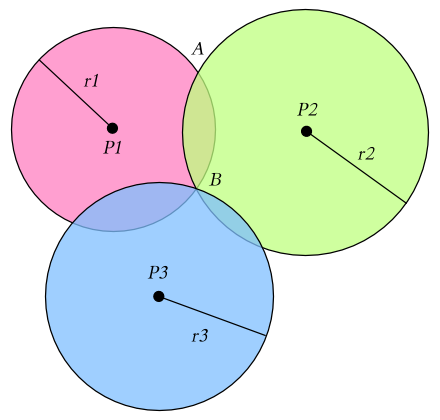
\includegraphics[width=0.5\linewidth]{assets/trilateration.png}
    \caption{Example of trilateration}
    \label{fig:trilateration}
\end{figure}

\subsection{RSSI-APIT Algorithm}

Research has shown that the RSSI-APIT localization algorithm achieves an average accuracy of 1.55 meters, reducing localization error by 57\% \cite{shen_indoor_2023}. However, it relies on the APIT framework, which requires numerous anchor points for effective functioning. In Shen et al. \cite{shen_indoor_2023}, 20 anchors were used to achieve these results. They found that at least 15 anchors are needed to maintain an error below 5 meters, and 20 anchors are required to reduce it to approximately 2 meters. Beyond 25 anchors, further improvements become negligible.   

Additionally, this algorithm requires training an artificial neural network, which presents challenges such as high data and energy consumption, as well as the need for retraining in different environments. As a result, the added accuracy does not justify the high setup, operational, and maintenance costs. 

\subsection{Machine learning based algorithms}

Significant research efforts aim to enhance Indoor Positioning System (IPS) accuracy using machine learning. However, surveys have failed to demonstrate clear advantages over traditional techniques. These methods remain limited in accuracy, reliability, scalability, and adaptability to diverse environments \cite{nessa_survey_2020}.   

The main benefit of machine learning approaches is their ability to make predictions without requiring explicit mathematical modeling—relying solely on observed data \cite{nessa_survey_2020}.

\subsection{Fingerprinting}

Fingerprinting-based localization requires an initial offline training phase before being used online \cite{nessa_survey_2020}, making it less scalable and adaptive. Constructing a radio map for localization involves substantial effort, particularly in large or dynamically changing environments \cite{nessa_survey_2020}. Furthermore, retraining is necessary when nodes are added or removed.   

K-Nearest Neighbors (K-NN) is the simplest algorithm applied for localization based on fingerprints. Recent research suggests that machine learning-enhanced fingerprinting methods, such as FPFE, can achieve a precision up to one meter. However, data collection is time-consuming and intensive. For example, Jiang et al. \cite{jiang_fingerprint_2021} required 2 minutes per reference point and over 6 hours for the complete dataset. Furthermore, any changes in the environment necessitate retraining, which can be impractical in dynamic settings like museums.

\subsection{Range-free localization techniques}

Some studies explore range-free techniques that do not rely on RSSI. However, they only become reliable in large environments with numerous devices. Chen et al. \cite{chen_range-free_2013} demonstrated this approach using 300 nodes across 40,000 square meters.  

\subsection{Summary}

In a museum setting, localization requires a balance between accuracy, stability, and ease of deployment. While fingerprinting and machine learning-based methods offer higher precision, their reliance on extensive pre-data collection and frequent retraining makes them impractical for dynamic environments where room layouts may change. Similarly, range-free techniques, which perform well in large-scale deployments, are not suitable for the relatively small indoor spaces of museums.  

Given these constraints, multi-lateration emerges as the most viable solution. Although it is an older technique, it remains a robust and resilient method that provides sufficient accuracy without the need for extensive calibration or high infrastructure costs. By relying on RSSI-based distance estimation from multiple beacons, multi-lateration offers a stable and cost-effective approach that aligns well with the requirements of a museum environment.

\section{Application in museums}

Only a few applications of Bluetooth Low Energy (BLE) in museums have been studied. For instance, \cite{barsocchi_detecting_2021} utilizes BLE beacons as proximity sensors, while \cite{verde_indoor_2023} focuses on determining a visitor's location within a specific room rather than identifying individual art pieces, enabling the delivery of relevant content in a broader context. 

In the realm of indoor localization, \cite{spachos_ble_2020} employed Kalman filtering to enhance distance estimation, achieving an error of less than 3.5 meters for 95\% of readings with raw data, and 3 meters with filtered data. This indicates that filtering uncertainties in raw data can significantly reduce average errors. The study found that when the receiver is within 50 centimeters of a beacon, the accuracy of the system is notably high, suggesting that positioning beacons close to Points of Interest (POIs) can enhance overall performance. Conversely, it is also noted that if beacons are spaced less than one meter apart, the accuracy may decrease.

\section{Summary}

This chapter has provided an overview of the main technologies and methods for indoor localization, with a particular focus on their applicability in museum environments. We compared the strengths and limitations of various approaches, including satellite navigation, QR codes, RFID, NFC, vision, infrared, ultrasound, ultra-wide band, Wi-Fi, Bluetooth, and hybrid systems. We also discussed key localization algorithms such as multi-lateration, RSSI-APIT, machine learning-based methods, fingerprinting, and range-free techniques. 

While no single technology or method is perfect, Bluetooth Low Energy (BLE) combined with multi-lateration offers a practical balance between accuracy, cost, and ease of deployment for museums. The review of related work highlights that, although BLE has been applied in some museum contexts, the field remains relatively underexplored, leaving room for further research and innovation. This background sets the stage for the following chapters, which will detail the design, implementation, and evaluation of a BLE-based indoor localization system tailored to the needs of museums.


